\documentclass[a4paper]{article}
\usepackage[spanish]{babel}
\usepackage[utf8]{inputenc}
\usepackage{graphicx}
\usepackage{pdfpages}
\usepackage{enumerate}
\usepackage{listings}
\usepackage{color}
\usepackage{indentfirst}
\usepackage{fancyhdr}
\usepackage{latexsym}
\usepackage[colorlinks=true, linkcolor=black]{hyperref}
\usepackage{wrapfig}
\usepackage{algpseudocode}
\usepackage{calc}
\usepackage{amsmath, amsthm, amssymb}
\usepackage{amsfonts}
\usepackage{lscape}
\definecolor{gray}{gray}{0.5}
\definecolor{light-gray}{gray}{0.95}
\definecolor{orange}{rgb}{1,0.5,0}

\usepackage{fancyhdr}
\pagestyle{fancy}

%\renewcommand{\chaptermark}[1]{\markboth{#1}{}}
\renewcommand{\sectionmark}[1]{\markright{\thesection\ - #1}}

\fancyhf{}

\fancyhead[LO]{Sección \rightmark} % \thesection\
\fancyfoot[LO]{\small{Leandro Matayoshi, Matías Pizzagalli, Gastón Requeni, Martín Santos}}
\fancyfoot[RO]{\thepage}
\renewcommand{\headrulewidth}{0.5pt}
\renewcommand{\footrulewidth}{0.5pt}
\setlength{\hoffset}{-0.8in}
\setlength{\textwidth}{16cm}
%\setlength{\hoffset}{-1.1cm}
%\setlength{\textwidth}{16cm}
\setlength{\headsep}{0.5cm}
\setlength{\textheight}{25cm}
\setlength{\voffset}{-0.7in}
\setlength{\headwidth}{\textwidth}
\setlength{\headheight}{13.1pt}

\renewcommand{\baselinestretch}{1.1}  % line spacing


\usepackage{underscore}
\usepackage{caratula}
\usepackage{url}

\newcommand{\cod}[1]{{\tt #1}}
\newcommand{\negro}[1]{{\bf #1}}
\newcommand{\ital}[1]{{\em #1}}
\newcommand{\may}[1]{{\sc #1}}
\newcommand{\tab}{\hspace*{2em}}

\newcommand{\sprintstory}[6]{\begin{tabular}{| p{3cm} | p{12cm} |}
 \hline
 TargetProcess ID: & #1 \\
 \hline
 User Story: & #2 \\
 \hline
 Esfuerzo estimado: & #3 \\
 \hline
 Business Value: & #4 \\
 \hline
 Descripción: & #5 \\
 \hline
 Criterios de\newline Aceptación: & #6 \\
 \hline
\end{tabular}}

\newcommand{\usecase}[3]{\noindent\textbf{CU\##1. #2}\\
#3\\
~\\
}

\newenvironment{taskstable}
{ \begin{tabular}{| p{14cm} | p{1cm} |}
 \hline
 \multicolumn{2}{|c|}{{\bf División en tareas}}\\
 \hline
 {\bf Tarea} & {\bf HH}\\
 \hline }
{ \end{tabular} }

\newcommand{\task}[2]{#1 & #2\\
 \hline}

\hypersetup{
 pdfstartview= {FitH \hypercalcbp{\paperheight-\topmargin-1in-\headheight}},
 pdfauthor={Grupo},
 pdfsubject={Dise\~{n}o}
}

\lstset{escapechar=@}

\begin{document}

\thispagestyle{empty}
\materia{Ingeniería de Software II}
\submateria{Primer Cuatrimestre de 2016}
\titulo{Trabajo Práctico II: The Curry Game release v7.1.2}

\integrante{Leandro Matayoshi}{79/11}{leandro.matayoshi@gmail.com}
\integrante{Matías Pizzagalli}{257/12}{matipizza@gmail.com}
\integrante{Gastón Requeni}{400/11}{grequeni@hotmail.com}
\integrante{Martín Santos}{413/11}{martin.n.santos@gmail.com}

\makeatletter

\maketitle

\newenvironment{myindentpar}[1]
{\begin{list}{1}
         {\setlength{\leftmargin}{#1}}
         \item[]
}
{\end{list}}

\newpage
\section{Casos de uso}
\begin{enumerate}
  \item Simulando desafío de basket según nuevas reglas
  \item Simulando desafíos de otros deportes
  \item Estableciendo estadísticas de jugadores de sitios oficiales y modificadas según redes sociales
  \item Participando en modo liga de fantasía. Usuario. 
  \item Participando en desafío o torneo grupal. Usuario.
  \item Chateando con otros participantes. Usuario.
  \item Posicionándose en ranking jerárquico. Usuario.
  \item Apostando dinero real en desafíos. Usuario.
  \item Controlando acceso de usuarios según leyes de la región respecto a apuestas online
  \item Mirando desafío ficticio en tiempo real. Usuario.
  \item Mirando en vivo partidos de ligas reales. Usuario.
  \item Agregando publicidad en el sitio
  \item Consultando datos estadísticos de usuarios de la aplicación
\end{enumerate}

\subsection{Descripción de los casos de uso, agrupados por área}

\subsubsection{Simulación}

\textbf{Simulando desafío de basket según las nuevas reglas}

Se refiere a modificar la simulación de forma tal que su duración sea similar a la de un partido real. Además incluye incorporar 
nuevas acciones, eventos y características del entorno que modifican la simulación: fouls, tiros libres, cambio de jugadores, cansancio
por minutos en cancha, estadios locales y visitantes, condiciones climáticas, movimientos de los jugadores y posiciones en cancha.

~

\textbf{Simulando desafíos de otros deportes}

Se refiere a la posibilidad de simular desafíos para diversos deportes

~

\textbf{Estableciendo estadísticas de jugadores de sitios oficiales y modificadas según redes sociales}

Se refiere a levantar las estadísticas de jugadores desde sitios oficiales y autorizados. Además las estadísticas
de los jugadores deberán modificarse en función de las menciones de los jugadores hechas en diversas redes sociales,
incluído el sistema de mensajería entre participantes.

\subsubsection{Desafíos}

\textbf{Participando en modo liga de fantasía. Usuario}

Se refiere a agregarle a los usuarios un modo en donde el resultado de los desafíos se definan según el desempeño de jugadores en partidos 
de ligas reales.

~

\textbf{Participando en desafío o torneo grupal. Usuario}

Se refiere a extender la modalidad de los desafíos de forma tal que puedan ser aceptados por varios jugadores. Estos desafíos corresponden a
un único partido, o varios de ellos. Al mismo tiempo pueden ser simulados o resolverse en el modo liga de fantasía.
Finalemnte, extender los desafíos de forma tal que también puedan ser creados por administradores del juego. 

~

\textbf{Chateando con otros participantes. Usuario}

Se refiere a agregar un servicio de mensajería que permita intercambiar mensajes tanto para participantes de un mismo desafío como para
amigos a través de la plataforma.

~

\textbf{Posicionándose en ranking jerárquico. Usuario}

Se refiere a posicionar a los jugadores en ranking jerárquicos: regionales, país, continente y mundial.
De esta manera los jugadores solo pueden acceder a desafíos acordes a su ranking. Este último se resetea cada año.

\subsubsection{Apuestas con dinero real}

\textbf{Apostando dinero real en desafíos. Usuario}

Se refiere a reemplazar el sistema de fichas ficticias por una suma de dinero real al momento de repartir premios por ganar desafíos.
Incluye agregar e integrar el sistema de pagos y cobros, y el ingreso de datos de tarjetas de crédito y cuentas bancarias al sistema.

~

\textbf{Controlando acceso de usuarios según leyes de la región respecto a apuestas online}

Se refiere a evitar el acceso de los usuarios al juego en países o regiones en donde las apuestas en los sitios de internet sean consideradas
ilegales, o bien permitir el registro de usuarios para que participen únicamente de los desafíos gratuitos.



\subsubsection{Streaming}

\textbf{Mirando desafío ficticio en tiempo real. Usuario}

Se refiere a que los usuarios puedan ver el minuto a minuto de los desafíos de forma gráfica. 
Subtareas: Elegir rendering 2D, 3D. Determinar rendering en función de la calidad óptima

~

\textbf{Mirando en vivo partidos de ligas reales. Usuario}

Se refiere a que los usuarios puedan ver desde la app o el sitio partidos de las ligas reales transmitidos en vivo.

\subsubsection{Publicidad y datos estadísticos}

\textbf{Agregando publicidad en el sitio}

Se refiere a desarrollar un mecanismo para que los sponsors e inversores de la aplicación puedan agregar publicidad de forma cómoda.

~

\textbf{Consultando datos estadísticos de usuarios de la aplicación}

Se refiere a la consulta de datos de los usuarios estadísticos por parte de inversores y sponsors para ser utilizados en futuras campañas publicitarias,
de marketing, etc. Los datos recolectados son de caracter demográfico, valor de las apuestas realizadas, jugador más seleccionado en los equipos, etc.


\newpage
\section{Análisis de riesgos}
A continuación presentamos un análisis de riesgos. Tuvimos en cuenta los riesgos más destacados, aunque cabe aclarar que este es un análisis inicial y los riesgos varían continuamente, por ende es posible que no sea completo.

\begin{figure}[h!]
  \centering
  \includegraphics[width=\textwidth]{imagenes/Riesgos.png}
  \caption{Tabla de riesgos. El color representa la exposición: Alta-Rojo, Media-Amarilla, Baja-Verde.}
\end{figure}


\subsection{Riesgos de exposición alta}

\noindent\textbf{R\#01: Robo de datos de tarjetas de crédito y/o bancarios [A] [A]} 
\begin{itemize}
	\item{\textbf{Descripción:} Dado que la aplicación será masiva y tendrá muchos datos de usuarios de todo el mundo, entonces (posiblemente) los datos de tarjetas de crédito y bancarios ingresados por los usuarios sean robados y/o publicados.}
	\item{\textbf{Probabilidad:} Alta, los hackers están muy interesados en esta información (más aún si es una aplicación masiva).}
	\item{\textbf{Impacto:} Alto. Ningún usuario volverá a utilizar la aplicación si se roban datos tan sensibles. Además el robo o la publicación de datos bancarios puede tener consecuencias muy graves tanto económicas como legales para el proyecto.}
	\item{\textbf{Mitigación:} Dedicarle el tiempo necesario (o más) al análisis y la elección de una arquitectura adecuada que permita persistir estos datos utilizando estrictas normas de seguridad. Pedir asesoramiento y trabajar conjuntamente con un equipo de expertos en seguridad informática y encriptación. Desarrollar este módulo lo antes posible para tener tiempo de contratar a terceros que lo auditen y lo prueben. Distribuír el almacenamiento de estos datos para reducir el impacto si uno de los servidores se ve comprometido.}
	\item{\textbf{Contingencia:} Bajar el sistema. Contratar a una empresa para que bloquee y denuncie los sitios que tengan plublicados los datos de nuestros usuarios. Tercerizar la búsqueda del error que permitió el robo de datos y la corrección.}
	\item{\textbf{Casos de uso afectados:} CU\#14, CU\#15, CU\#16}
\end{itemize}

~

\noindent\textbf{R\#02: Interrupción del streaming por falla de red [A] [A] } 
\begin{itemize}
	\item{\textbf{Descripción:} Dado que las fallas de red ocurren habitualmente, entonces (posiblemente) la red falle e interrumpa el streaming de un partido.}
	\item{\textbf{Probabilidad:} Alta.}
	\item{\textbf{Impacto:} Alto, dado que puede implicar la pérdida de usuarios.}
	\item{\textbf{Mitigación:} Construir una red que tenga caminos alternativos y garantice alta disponibilidad. Es muy importante que la arquitectura tenga esto en cuenta para que la caída de un tramo de la red no impacte demasiados usuarios (preferentemente ninguno).}
	\item{\textbf{Contingencia:} Contratar servicios externos como YouTube o Vimeo para realizar streaming de partidos mientras se solucionan problemas de red.}
	\item{\textbf{Casos de uso afectados:} CU\#6, CU\#9}
\end{itemize}

~

\noindent\textbf{R\#03: Streaming de video imposibilitado por falta de ancho de banda [A] [A]} 
\begin{itemize}
	\item{\textbf{Descripción:} Dado que los anchos de banda de las conexiones son muy distintos a lo largo del mundo y que un stream de video consume mucho ancho de banda, entonces (posiblemente) los usuarios no puedan ver los desafíos debido a que el streaming requiere de una cantidad de datos mayor a la soportada por la conexión.}
	\item{\textbf{Probabilidad:} Alta.}
	\item{\textbf{Impacto:} Alto. Los usuarios desean ver los desafíos en la mayor calidad posible, pero estarán muy disconformes si no pueden hacerlo en absoluto. Potencialmente dejarán la aplicación por este problema.}
	\item{\textbf{Mitigación:} Dedicarle el tiempo necesario (o más) al análisis y la elección  de una arquitectura adecuada que permita transmitir muchos datos. Hacer un análisis profundo del estado de conectividad de cada región en donde desea lanzarse el producto. Elegir la resolución en función del análisis realizado. Implementar mecanismos de autoadaptación de bitrate según ancho de banda (considerando posibles congestiones en la red).}
	\item{\textbf{Contingencia:} En las regiones donde se hayan producido las fallas, bajar el bitrate al mínimo para garantizar que puedan ser vistos los partidos (con baja calidad).}
	\item{\textbf{Casos de uso afectados:} }
\end{itemize}

~

\noindent\textbf{R\#04: Hackean y modifican el código de un módulo de simulación [A] [A] } 
\begin{itemize}
	\item{\textbf{Descripción:} Dado que los módulos de simulación determinan un ganador por partido y a fin de cuentas esto se traduce en algún premio o compensación para un participante, entonces (posiblemente) haya hackers que intenten atacarnos y alterar el código fuente de los módulos de simulación para beneficiarse en el juego.}
	\item{\textbf{Probabilidad:} Alta.}
	\item{\textbf{Impacto:} Alto.}
	\item{\textbf{Mitigación:} Usar hash de código fuente y verificarlo con cierta frecuencia para reducir la probabilidad de que esto no sea detectado a tiempo. También debemos configurar correctamente firewall y protocolos de transferencia de datos para evitar alteraciones en las simulaciones.}
	\item{\textbf{Contingencia:} Hacer un nuevo deploy del módulo alterado y desactivar las cuentas de los participantes beneficiados. No les podemos quitar los premios a menos que podamos demostrar culpabilidad según las leyes de la región.}
	\item{\textbf{Casos de uso afectados:} CU\#6}
\end{itemize}

~

\noindent\textbf{R\#05: Pérdida de datos estadísticos históricos de participantes usados para minería de datos [M] [A] } 
\begin{itemize}
	\item{\textbf{Descripción:} Dado que cualquier medio de almacenamiento físico podría dañarse, entonces (posiblemente) perderíamos los datos estadísticos históricos de participantes que nuestros sponsors utilizan para minar datos.}
	\item{\textbf{Probabilidad:} Media.}
	\item{\textbf{Impacto:} Alto. El sistema seguirá funcionado, pero los sponsors perderán dinero y corre riesgo la continuidad del proyecto.}
	\item{\textbf{Mitigación:} Priorizar la redundancia de estos datos porque son críticos para que el proyecto genere mucha ganancia monetaria.}
	\item{\textbf{Contingencia:} Según el nivel de péridida de los datos, evaluar posibles compensaciones volviendo a ejecutar simulaciones o recalculando resultados.}
	\item{\textbf{Casos de uso afectados:} CU\#22, CU\#23}
\end{itemize}

~

\noindent\textbf{R\#06: Pérdida parcial o total del log de facturación [M] [A] } 
\begin{itemize}
	\item{\textbf{Descripción:} Dado que el fisco de las distintas regiones podría exigirnos presentar declaraciones juradas con los montos detallados de facturación y dado que ese detalle se guarda en almacenamiento físico propenso a fallas, entonces (posiblemente) podría perderse parcial o totalmente.}
	\item{\textbf{Probabilidad:} Media.}
	\item{\textbf{Impacto:} Alto. No sólo afectaría legalmente al proyecto en las regiones más estrictas, sino que además los sponsors no podrían acceder al estado de cuenta detallado por región (sólo nos quedaría usar las cuentas bancarias, pero sin el detalle generado por nosotros).}
	\item{\textbf{Mitigación:} Priorizar la redundancia de estos datos y regionalizar el log. Esto bajaría la probabilidad de perder datos (porque deberían perderse todas las copias) pero además reduce el impacto (porque si se pierde, se perderá sólo de una región y no de todo el mundo).}
	\item{\textbf{Contingencia:} Usar datos de entidades bancarias que manejan las cuentas de los sponsors y de facturación propia de la aplicación para reconstruir los datos de facturación (aunque perdamos detalles).}
	\item{\textbf{Casos de uso afectados:} CU\#16}
\end{itemize}

~

\noindent\textbf{R\#07: Mal desempeño del render 3D de la simulación en tiempo real [A] [M] } 
\begin{itemize}
	\item{\textbf{Descripción:} Dado que hay una inmensa variedad de dispositivos que van a ejecutar nuestra aplicación, entonces (posiblemente) en algunos de ellos se produzca un mal desempeño del render 3D de la simulación que impida el seguimiento del partido en tiempo real.}
	\item{\textbf{Probabilidad:} Alta.}
	\item{\textbf{Impacto:} Medio, dado que implica pérdida de los seguidores más exigentes de calidad en todo el segmento de dispositivos que no soportan la simulación.}
	\item{\textbf{Mitigación:} Desarrollar un módulo que detecte la capacidad del dispositivo de utilizar el render 3D, y en caso que no lo soporte utilizar el render 2D.}
	\item{\textbf{Contingencia:} Transmitir el partido con render 2D para que todos puedan verlo y mientras tanto analizar cómo solucionar el problema en futuras transmisiones.}
	\item{\textbf{Casos de uso afectados:} CU\#6}
\end{itemize}

\subsection{Riesgos de exposición media}

\noindent\textbf{R\#08: Imposibilidad de obtener estadísticas de partido/jugadores reales en tiempo real [B] [A] } 
\begin{itemize}
	\item{\textbf{Descripción:} Dado que las estadísticas para usar en simulaciones y en ligas de fantasía se obtienen de un proveedor externo, entonces (posiblemente) pueda fallar el servidor del proveedor y dejaría de funcionar el juego por no poder obtener los datos estadísticos.}
	\item{\textbf{Probabilidad:} Baja, dado que utilizaremos servicios populares que tienen años de experiencia y funcionamiento sin fallas.}
	\item{\textbf{Impacto:} Alto, ya que dejaría de funcionar cualquier simulación o desafíos de liga de fantasía.}
	\item{\textbf{Mitigación:} En caso de falla al obtener datos, realizar reintentos. Si los reintentos fallan, utilizar los últimos datos recibidios. Al mismo tiempo, disparar alarmas a los responsables para intentar solucionar el problema antes de que impacte el juego de manera irreversible.}
	\item{\textbf{Contingencia:} Si el juego debe dejar de funcionar porque pasó mucho tiempo sin obtener datos estadísticos nuevos, se deberá resolver el problema lo antes posible y mientras tanto indicar a los participantes que el sitio se encuentra en mantenimiento.}
	\item{\textbf{Casos de uso afectados:} CU\#6, CU\#9}
\end{itemize}

~

\noindent\textbf{R\#09: Hackean el servidor del proveedor de datos estadísticos [B] [A] } 
\begin{itemize}
	\item{\textbf{Descripción:} Dado que desconocemos las medidas de seguridad usadas por los proveedores de datos estadísticos de partidos, entonces (posiblemente) lo hackeen y modifiquen todos los datos, impactando nuestras simulaciones y resultados de liga de fantasía.}
	\item{\textbf{Probabilidad:} Baja. Los proveedores tienen mucha trayectoria y experiencia y no hay registros de hackeos.}
	\item{\textbf{Impacto:} Alto. Podrían entregarse muchos premios a las personas equivocadas y potencialmente muchos usuarios dejarán de usar la aplicación.}
	\item{\textbf{Mitigación:} Auditoría de la seguridad de los sistemas del proveedor.}
	\item{\textbf{Contingencia:} Suspender todos los partidos y reversar pagos. En un caso tan extremo, todos los premios deberían desestimarse, así como las cuotas de entrada a desafíos en vigencia deberían devolverse.}
	\item{\textbf{Casos de uso afectados:} CU\#6, CU\#9}
\end{itemize}

~

\noindent\textbf{R\#10: Se produce un corte masivo en la red que impide que la mayoría de los usuarios puedan acceder al juego [B] [A] } 
\begin{itemize}
	\item{\textbf{Descripción:} Dado que el juego se accede via internet y se puede acceder en todo el mundo gracias a nuestra infraestructura de red, entonces (posiblemente) se produzca un corte masivo en la red que impida que la mayoría de los usuarios puedan acceder al juego.}
	\item{\textbf{Probabilidad:} Baja.}
	\item{\textbf{Impacto:} Alto. Se pierde mucho dinero.}
	\item{\textbf{Mitigación:} Garantizar alta disponibilidad de nuestro sistema en todos los aspectos funcionales.}
	\item{\textbf{Contingencia:} Actuar lo más rápido posible. Contratar temporalmente servidores de Google y Amazon para volver a poner el juego online.}
	\item{\textbf{Casos de uso afectados:} Todos los casos de uso relacionados al participante.}
\end{itemize}

~

\noindent\textbf{R\#11: Rediseño de la versión anterior del simulador de basquet [M] [M]}
\begin{itemize}
	\item{\textbf{Descripción:} Dado que la versión anterior del simulador puede no ser lo suficientemente extensible/modificable como para poder incorporar los cambios requeridos, entonces (posiblemente) haya que realizar un profundo rediseño y se atrase el proyecto.}
	\item{\textbf{Probabilidad:} Media}
	\item{\textbf{Impacto:} Medio, ya que retrasaría la fecha del release del producto. Los usuarios quieren poder ver estos detalles y nuevas acciones en las simulaciones.}
	\item{\textbf{Mitigación:} Evaluar extensibilidad del diseño para los nuevos requerimientos en el momento de la estimación y asignar la realización de este módulo a la primer etapa de la construcción para evitar posibles retrasos en la fecha de entrega (No se incluye en la etapa de la elaboración ya que está relacionado con la funcionalidad y no con la arquitectura)}
	\item{\textbf{Contingencia:} Hacer el rediseño pensando en funcionalidad y no tanto en un buen diseño, priorizando cumplir con los tiempos.}
	\item{\textbf{Casos de uso afectados:} CU\#6}
\end{itemize}

~

\noindent\textbf{R\#12: Cambia un dato estadístico en tiempo real por un error (ej: se anula un gol) y se paga por error a un participante en un desafío de liga de fantasía [M] [M] } 
\begin{itemize}
	\item{\textbf{Descripción:} Dado que los datos usados para resolver jugadas en los simuladores provienen de proveedores externos en tiempo real, entonces (posiblemente) podría cambiar un dato (ej: se anula un gol) y en la liga de fantasía podría estar pagándose un premio por error.}
	\item{\textbf{Probabilidad:} Media.}
	\item{\textbf{Impacto:} Medio. Esto implicaría una pérdida de dinero ya que no se puede pedir a un participante que devuelva el premio.}
	\item{\textbf{Mitigación:} Antes de pagar premios dejar pasar un tiempo prudencial (de 10 minutos a 1 hora) para que los datos tengan más confiabilidad y luego sí utilizarlos.}
	\item{\textbf{Contingencia:} Suspender el pago de premios de liga de fantasía y agregar nuevas validaciones. Contactar al proveedor y solicitar reducción de frecuencia de fallas.}
	\item{\textbf{Casos de uso afectados:} }
\end{itemize}

~

\noindent\textbf{R\#13: Contratiempos en el desarrollo de simuladores de otros deportes [M] [M]}
\begin{itemize}
	\item{\textbf{Descripción:} Dado que el desarrollo de un simulador para otro deporte (que no sea basquet) puede requerir contemplar situaciones que no han surgido hasta el momento (dado que el dominio es desconocido para los desarrolladores), entonces (posiblemente) surjan contratiempos en el desarrollo de los nuevos simuladores y se atrase el proyecto.}
	\item{\textbf{Probabilidad:} Media}
	\item{\textbf{Impacto:} Medio, ya que retrasaría la fecha del release del producto}
	\item{\textbf{Mitigación:} Si bien resulta razonable tomar por cota superior el tiempo que ha tomado el desarrollo del simulador de basquet para estimar el tiempo de los demás simuladores, estimar un adicional del 20\% del tiempo para cualquier eventualidad}
	\item{\textbf{Contingencia:} Sacar un primer release con menos features de los simuladores para cumplir con la entrega y planificar las mejoras con más tiempo.}
	\item{\textbf{Casos de uso afectados:} CU\#6}
\end{itemize}

~

\noindent\textbf{R\#14: Falla un engine 3D o 2D [M] [M] } 
\begin{itemize}
	\item{\textbf{Descripción:} Dado que los engines 3D y 2D son desarrollados por un proveedor tercerizado, entonces (posiblemente) el software tenga errores y falle en algunos o todos los dispositivos bajo ciertas circunstancias.}
	\item{\textbf{Probabilidad:} Media.}
	\item{\textbf{Impacto:} Medio. La simulación no va a fallar, sólo la renderización, pero esto podría provocar que los usuarios dejen de usar la aplicación porque no les anda.}
	\item{\textbf{Mitigación:} Tercerizar el testing y análisis de los renderizadores 3D y 2D.}
	\item{\textbf{Contingencia:} Utilizar streaming de video en todos los casos (deshabilitar el uso de los engines), hasta que el proveedor corrija el problema.}
	\item{\textbf{Casos de uso afectados:} CU\#6}
\end{itemize}

~

\noindent\textbf{R\#15: Funcionar de forma ilegal en una región [M] [M] } 
\begin{itemize}
	\item{\textbf{Descripción:} Dado que en algunas regiones hay restricciones con respecto a juegos/apuestas online, podría pasar que el sistema funcione de forma ilegal en una región.}
	\item{\textbf{Probabilidad:} Media.}
	\item{\textbf{Impacto:} Medio. Pueden generarse inconvenientes económicos y legales pero la aplicación no dejará de funcionar en las demás regiones donde sí es legal.}
	\item{\textbf{Mitigación:} Realizar pruebas de filtrado de IP en conjunto con empresas de seguridad informática. Desarrollar un módulo de detección de accesos vía proxies y VPNs y bloquearlos. Realizar una reunión con dpto. de seguridad informática de Netflix (que ya tuvieron este problema).}
	\item{\textbf{Contingencia:} Detectar cómo se logró el acceso al sitio (o a funcionalidades del mismo) desde una región no permitida y desarrollar módulos de defensa de ese punto débil.}
	\item{\textbf{Casos de uso afectados:} CU\#1, CU\#2, CU\#3, CU\#18, CU\#20}
\end{itemize}

\subsection{Riesgos de exposición baja}

\noindent\textbf{R\#16: Mal desempeño del render 2D de la simulación en tiempo real [B] [M] } 
\begin{itemize}
	\item{\textbf{Descripción:} Dado que hay una inmensa variedad de dispositivos que van a ejecutar nuestra aplicación, entonces (posiblemente) en algunos de ellos se produzca un mal desempeño del render 2D de la simulación que impida el seguimiento del partido en tiempo real.}
	\item{\textbf{Probabilidad:} Baja.}
	\item{\textbf{Impacto:} Medio, dado que implica pérdida de los seguidores más exigentes de calidad en todo el segmento de dispositivos que no soportan la simulación.}
	\item{\textbf{Mitigación:} Desarrollar un módulo que detecte la capacidad del dispositivo de utilizar el render 2D, y en caso que no lo soporte utilizar streaming de video.}
	\item{\textbf{Contingencia:} Transmitir el partido como stream de video para que todos puedan verlo y mientras tanto analizar cómo solucionar el problema en futuras transmisiones.}
	\item{\textbf{Casos de uso afectados:} CU\#6}
\end{itemize}

~

\noindent\textbf{R\#17: Se cae la transmisión en vivo de partidos reales [B] [M]} 
\begin{itemize}
	\item{\textbf{Descripción:} Dado que dependemos de un proveedor externo para transmitir partidos reales en vivo, entonces (posiblemente) ocurra una falla y se caiga la transmisión.}
	\item{\textbf{Probabilidad:} Baja.}
	\item{\textbf{Impacto:} Medio. Los más fanáticos se van a enojar mucho si se pierden una anotación de su equipo.}
	\item{\textbf{Mitigación:} Firmar un contrato con las empresas de televisación de partidos que nos garantice 99,99\% de disponibilidad de sus transmisiones.}
	\item{\textbf{Contingencia:} Ofrecer un video del partido a los usuarios afectados para que puedan volver a ver el partido sin cortes.}
	\item{\textbf{Casos de uso afectados:} CU\#9}
\end{itemize}

~

\noindent\textbf{R\#18: Cambia un dato estadístico en tiempo real por un error (ej: se anula un gol) y la simulación utiliza información errónea para determinar resultados de jugadas [M] [B] } 
\begin{itemize}
	\item{\textbf{Descripción:} Dado que los datos usados para resolver jugadas en los simuladores provienen de proveedores externos en tiempo real, entonces (posiblemente) podría cambiar un dato (ej: se anula un gol) y la simulación quizás ya había usado la versión anterior del dato (que era errónea).}
	\item{\textbf{Probabilidad:} Media.}
	\item{\textbf{Impacto:} Bajo. Sólo se verán afectadas ciertas jugadas, que no deberían modificar demasiado el resultado final del partido.}
	\item{\textbf{Mitigación:} Firmar un contrato de calidad de datos con los proveedores, que garantice que el 99,99\% de las consultas devuelvan datos sin errores o previamente validados en los casos más críticos, aunque esto represente una demora en la obtención.}
	\item{\textbf{Contingencia:} Si la diferencia del resultado es muy notoria, anular el partido. Si se repiten estas situaciones, evaluar una estrategia de mediación entre los participantes del partido cuyo resultado se vio afectado para resolver el problema.}
	\item{\textbf{Casos de uso afectados:} CU\#6, CU\#9}
\end{itemize}

~

\noindent\textbf{R\#19: Un simulador no es aprobado en una región por sospecha de fraude [B] [B] } 
\begin{itemize}
	\item{\textbf{Descripción:} Dado que un auditor de cada país evaluará nuestros simuladores para verificar que no haya fraude, entonces (posiblemente) no nos aprueben uno de los simuladores porque se considera fraudulento (aunque no necesariamente lo sea).}
	\item{\textbf{Probabilidad:} Baja.}
	\item{\textbf{Impacto:} Bajo. Los fanáticos de ese deporte no podrán simular partidos. Perderíamos algunos clientes.}
	\item{\textbf{Mitigación:} Enviar gente capacitada junto con el código fuente para explicar detalles de funcionamiento frente a los auditores y así evitar falsas interpretaciones del código. En el peor caso, esta gente puede persuadir al auditor...}
	\item{\textbf{Contingencia:} Se buscará bloquear ciertas partes del funcionamiento o crear un simulador especial para la región si la cantidad de clientes es considerable (esta cantidad se puede determinar en base al uso de la liga de fantasía de ese deporte en esa misma región).}
	\item{\textbf{Casos de uso afectados:} CU\#6}
\end{itemize}












% \textbf{Caso de uso \#1:} Simulando desafío de basket según nuevas reglas
% \begin{itemize}
% \item{\textbf{Riesgo:} La versión anterior del simulador puede no ser lo suficientemente extensible/modificable como para poder incorporar los cambios requeridos, lo cual
% puede implicar un profundo rediseño}
% \item{\textbf{Contingencia:} Asignar la realización de este caso de uso a la primer etapa de la construcción para evitar posibles retrasos en la fecha de entrega. (No se incluye
% en la etapa de la elaboración ya que está relacionado con la funcionalidad y no con la arquitectura)}
% \item{\textbf{Probabilidad:} Media}
% \item{\textbf{Impacto:} Medio, ya que retrasaría la fecha del release del producto. Los usuarios quieren poder ver estos detalles y nuevas acciones en las simulaciones.}
% \end{itemize}

% ~

% \textbf{Caso de uso \#2:} Simulando desafíos de otros deportes
% \begin{itemize}
% \item{\textbf{Riesgo:} Dominio desconocido: Pueden generarse contratiempos en el desarrollo de los simuladores de otro deporte, al ser escencialmente diferentes al basket}
% \item{\textbf{Descripción:} El equipo de desarrollo cuenta con cierta experiencia previa ya que ha implementado el simulador de basket. Sin embargo, el desarrollo de
% un simulador para otro deporte puede requerir contemplar situaciones que no han surgido hasta el momento}
% \item{\textbf{Mitigación:} Si bien resulta razonable tomar por cota superior el tiempo que ha tomado el desarrollo del simulador de basket para estimar el tiempo de los 
% demás simuladores, estimar un adicional del 20\% del tiempo para cualquier eventualidad}
% \item{\textbf{Probabilidad:} Media}
% \item{\textbf{Impacto:} Medio, ya que retrasaría la fecha del release del producto}
% \end{itemize}

% ~

% \textbf{Caso de uso \#7:} Posicionándose en ranking jerárquico. Usuario.
% \begin{itemize}
% \item{\textbf{Riesgo:} La mala elección de la arquitectura o de la distribución de los servidores puede degradar gravemente la performance. La correcta implementación de este caso de uso es vital para el 'core' de la aplicación, debido a la masiva cantidad de usuarios que tenga el sistema}
% \item{\textbf{Contingencia:} Asignarle al desarrollo de este caso de uso un papel central en el proceso. Dedicarle el tiempo necesario (o más) al análisis y la elección 
% de una arquitectura adecuada, una posible distribución de servidores y la elección de empresas que nos provean de dichos servidores vs la compra de servidores. Se le ha asignado
% un lugar en la 1ra iteración del proceso de elaboración}
% \item{\textbf{Probabilidad:} Alta}
% \item{\textbf{Impacto:} Alto. Una performance degradada a nivel general puede implicar graves riesgos para el producto}
% \end{itemize}

% ~

% \textbf{Caso de uso \#8:} Apostando dinero real en desafíos. Usuario.
% \begin{itemize}
% \item{\textbf{Riesgo:} Los datos de tarjetas de crédito y bancarios ingresados por los usuarios pueden ser robados o publicados. Se está trabajando con data extremadamente
% sensible}
% \item{\textbf{Contingencia:} Asignarle al desarrollo de este caso de uso un papel central en el proceso. Dedicarle el tiempo necesario (o más) al análisis y la elección 
% de una arquitectura adecuada que permita persistir estos datos utilizando estrictas normas de seguridad. Pedir asesoramiento y trabajar conjuntamente con un equipo de expertos en seguridad informática y encriptación. Se le ha asignado un lugar en la 2da iteración del proceso de elaboración}
% \item{\textbf{Probabilidad:} Alta}
% \item{\textbf{Impacto:} Alto. El robo o la publicación de datos bancarios puede tener consecuencias muy graves tanto económicas como legales para el proyecto}
% \end{itemize}

% ~

% \textbf{Caso de uso \#9:} Controlando acceso de usuarios según leyes de la región respecto a apuestas online
% \begin{itemize}
% \item{\textbf{Riesgo:} Actuar de forma ilegal en aquellas regiones en donde las apuestas están prohibidas}
% \item{\textbf{Contingencia:} Reflexionar en conjunto con el caso de uso \textbf{\#8}} 
% \item{\textbf{Probabilidad:} Media}
% \item{\textbf{Impacto:} Medio. Pueden generarse inconvenientes económicos y legales}
% \end{itemize}

% ~

% \textbf{Caso de uso \#10 y \#11:} Streaming de desafíos
% \begin{itemize}
% \item{\textbf{Riesgo:} Los usuarios no pueden ver los desafíos debido a que el streaming requiere de una cantidad de datos mayor a la soportada por la conexión}
% \item{\textbf{Contingencia:} Asignarle al desarrollo de este caso de uso un papel central en el proceso. Dedicarle el tiempo necesario (o más) al análisis y la elección 
% de una arquitectura adecuada que permita transmitir muchos datos. Hacer un análisis profundo del estado de conectividad de cada región en donde desea lanzarse el prodcuto.
% Elegir el rendering en 2D/3D en función del análisis. Para el caso del streaming de los partidos reales, elegir la resolución en función del análisis realizado}
% \item{\textbf{Probabilidad:} Alta}
% \item{\textbf{Impacto:} Medio. Los usuarios desean ver los desafíos en la mayor calidad posible, pero estarán muy disconformes si no pueden hacerlo en absoluto}
% \end{itemize}


% \subsection{Tabla de análisis de riesgos}

% \begin{center}
%     \begin{tabular}{ | l | l | l | p{5cm} |}
%     \hline
%     Impacto | Probabilidad & Alta & Media & Baja \\ \hline
%     Alto & (7)-(8) & - & - \\ \hline
%     Medio & (10)-(11) & (1)-(2)-(9) & - \\ \hline
%     Bajo & - & - & - \\ \hline
%     \end{tabular}
% \end{center}

\newpage
\section{WBS}
En el proceso de elaboración se incluyen las tareas relacionadas con la arquitectura del sistema, y se genera una base ejecutable del código sobre la cual se pueda 
empezar a testear dicha arquitectura.

Al mismo tiempo se desarrollan los componentes con un rol central dentro de la arquitectura definida, y los módulos de los casos de uso con más riesgos
de alto impacto a nivel estructural, dejando cada una en una iteración diferente. La idea es construir la arquitectura de forma incremental. La opción a nivel arquitectura propuesta
en cada iteración debe ser compatible con la anterior, y al mismo tiempo solucionar el caso de uso actual.

\begin{figure}[h!]
   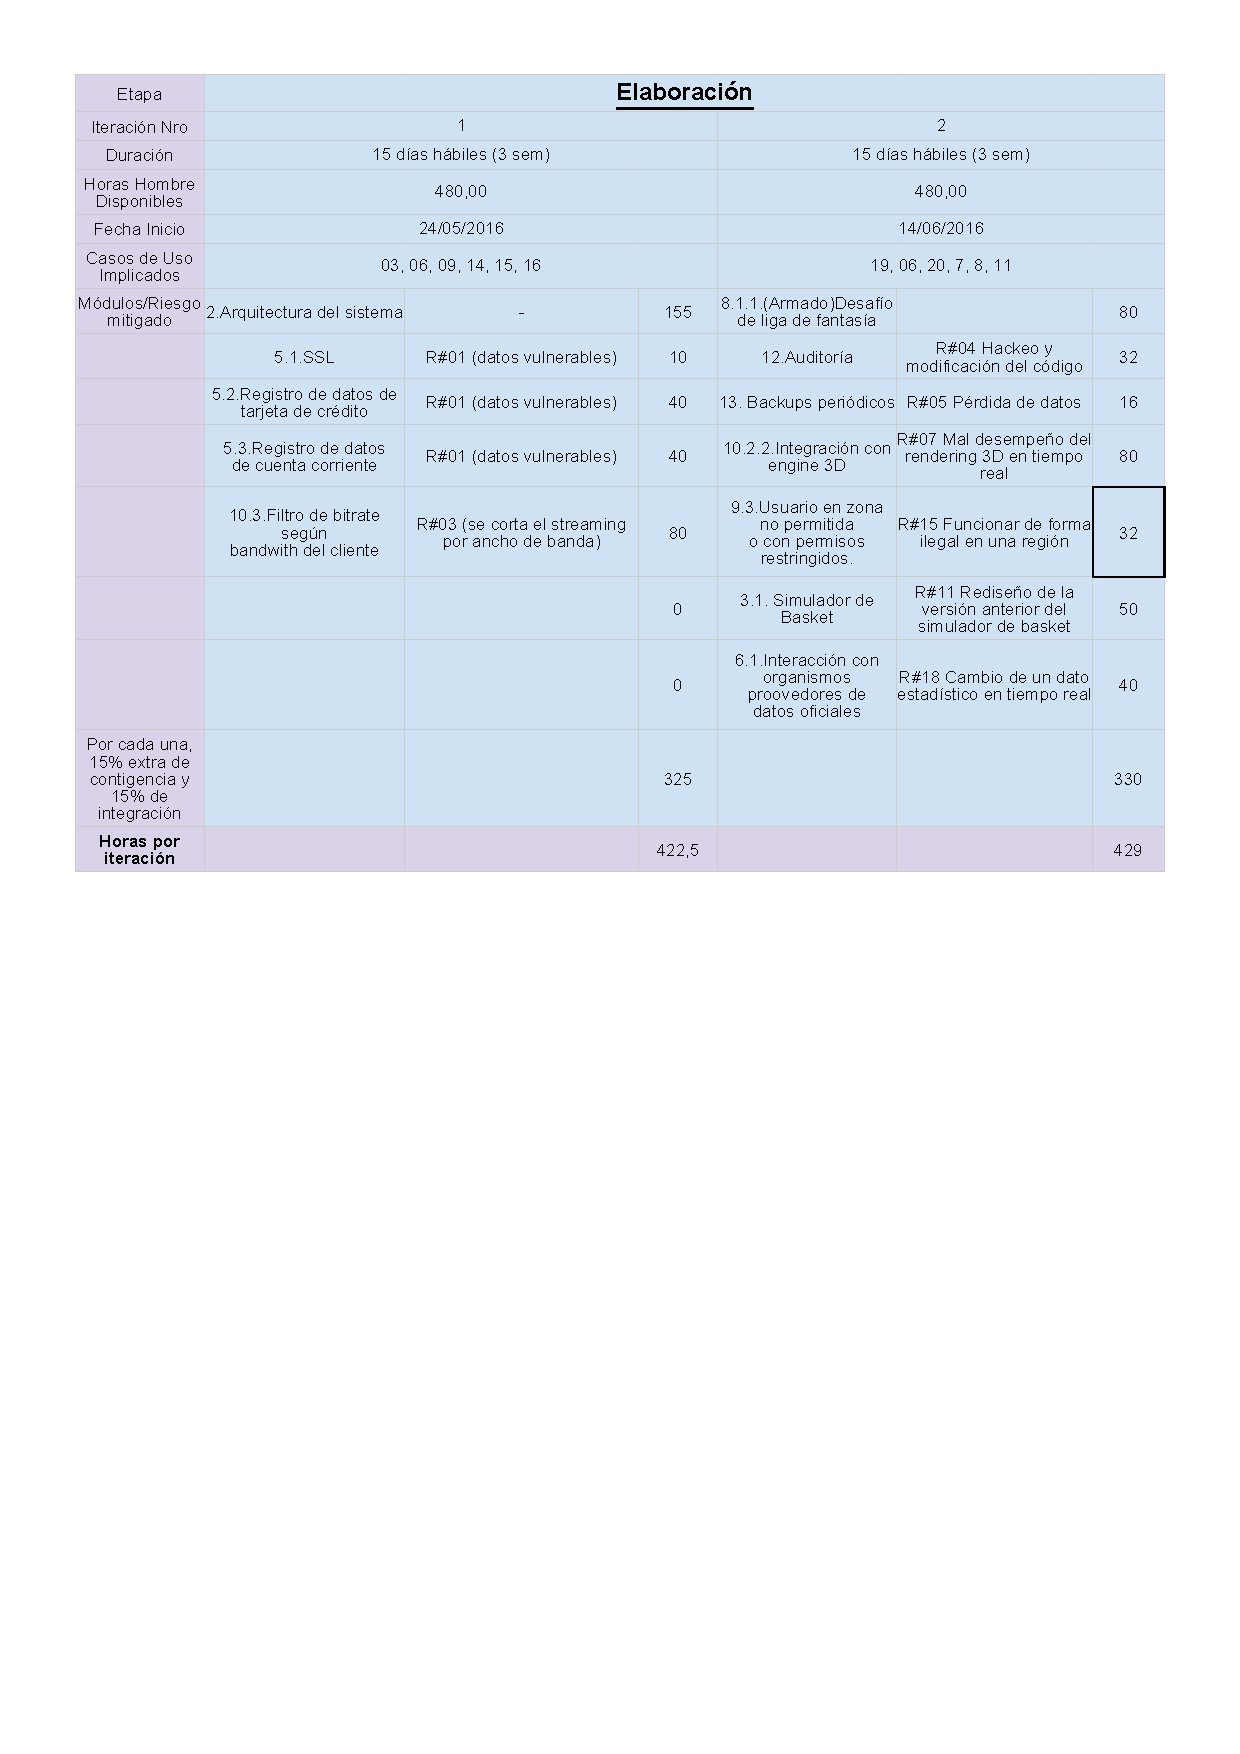
\includegraphics[scale=0.80]{imagenes/etapas-elaboracion.pdf}
   \caption{División de tareas en la etapa de elaboración}
\end{figure}

En la etapa de construcción se desarrollan los módulos y casos de uso faltantes faltantes de forma iterativa incremental. 

Finalmente en la etapa de transición se realizan tareas de mantenimiento.

\newpage
\begin{landscape}

\begin{figure}[h!]
   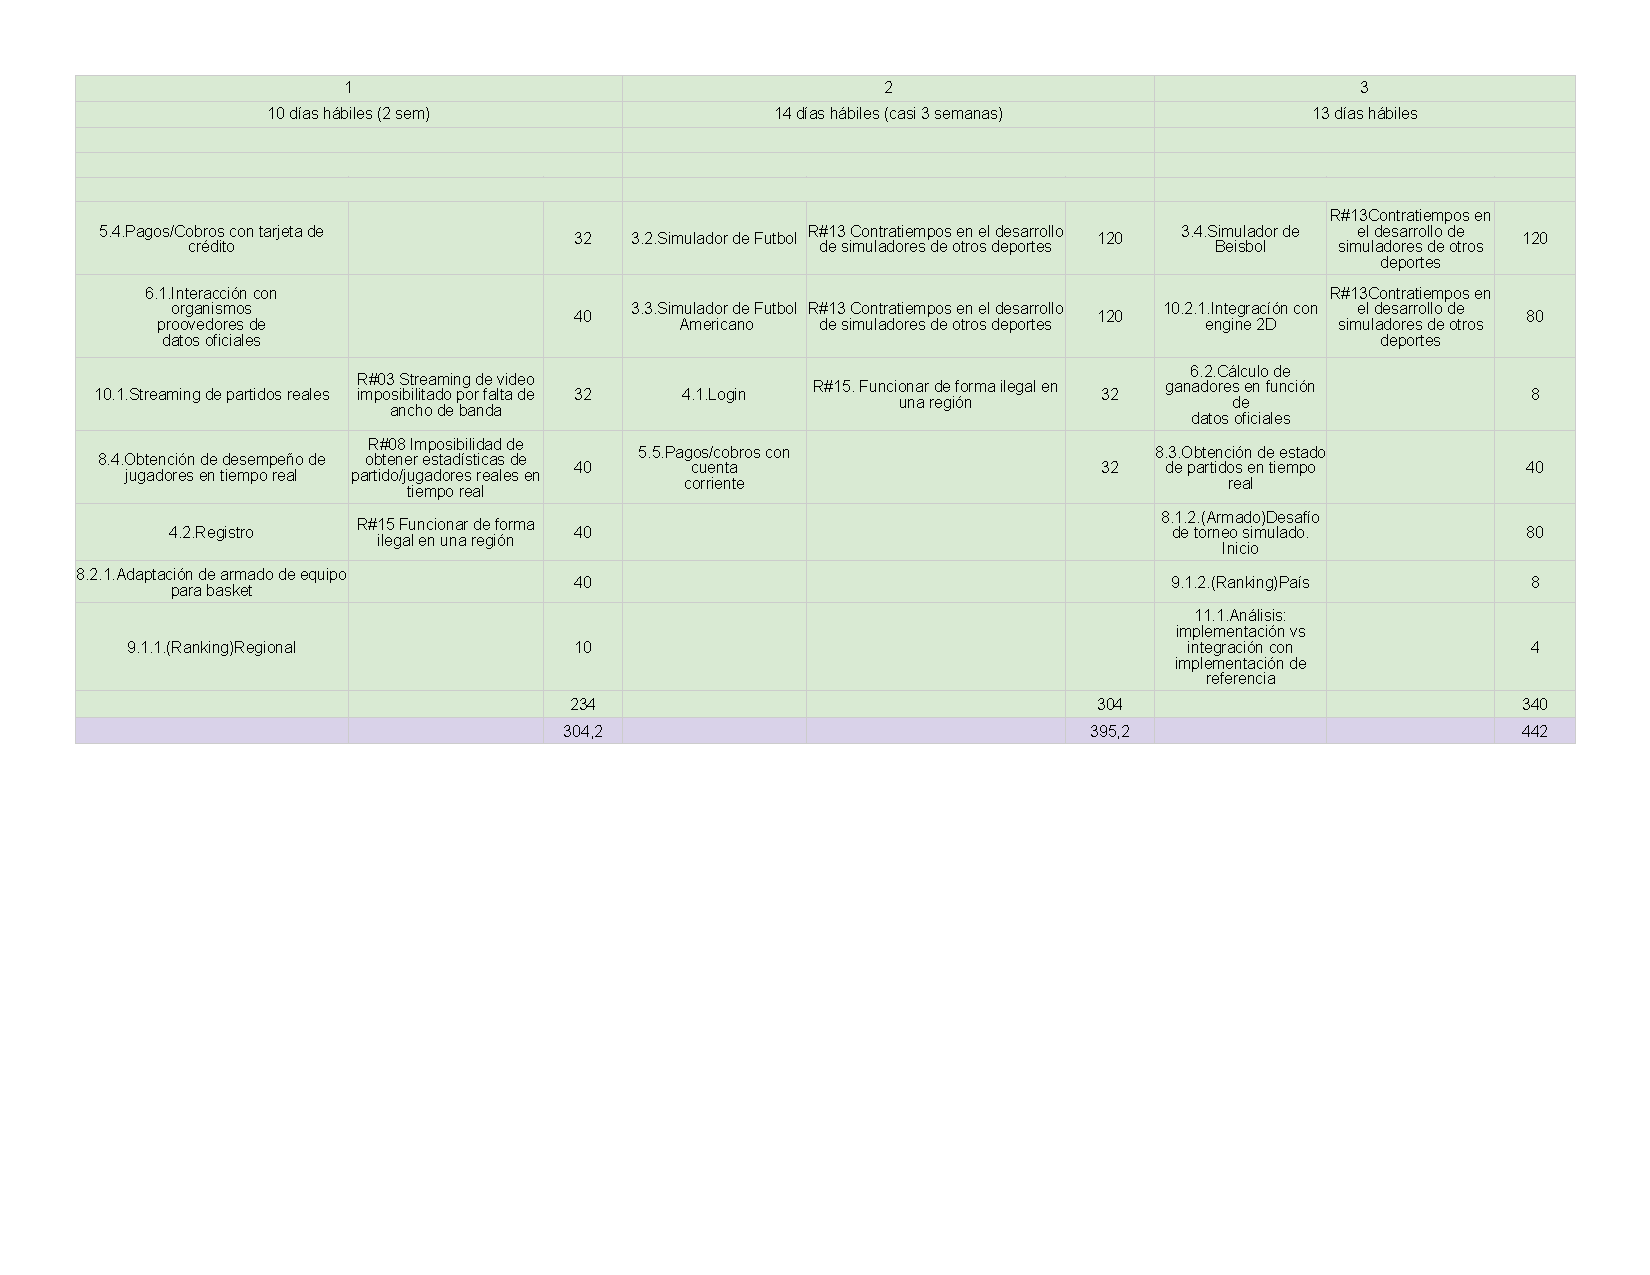
\includegraphics[scale=0.8]{imagenes/construccion123.pdf}
   \caption{División de tareas de las primeras 3 iteraciones de la etapa de 'Construcción'}
\end{figure}

\end{landscape}
\newpage

\newpage
\begin{landscape}

\begin{figure}[h!]
   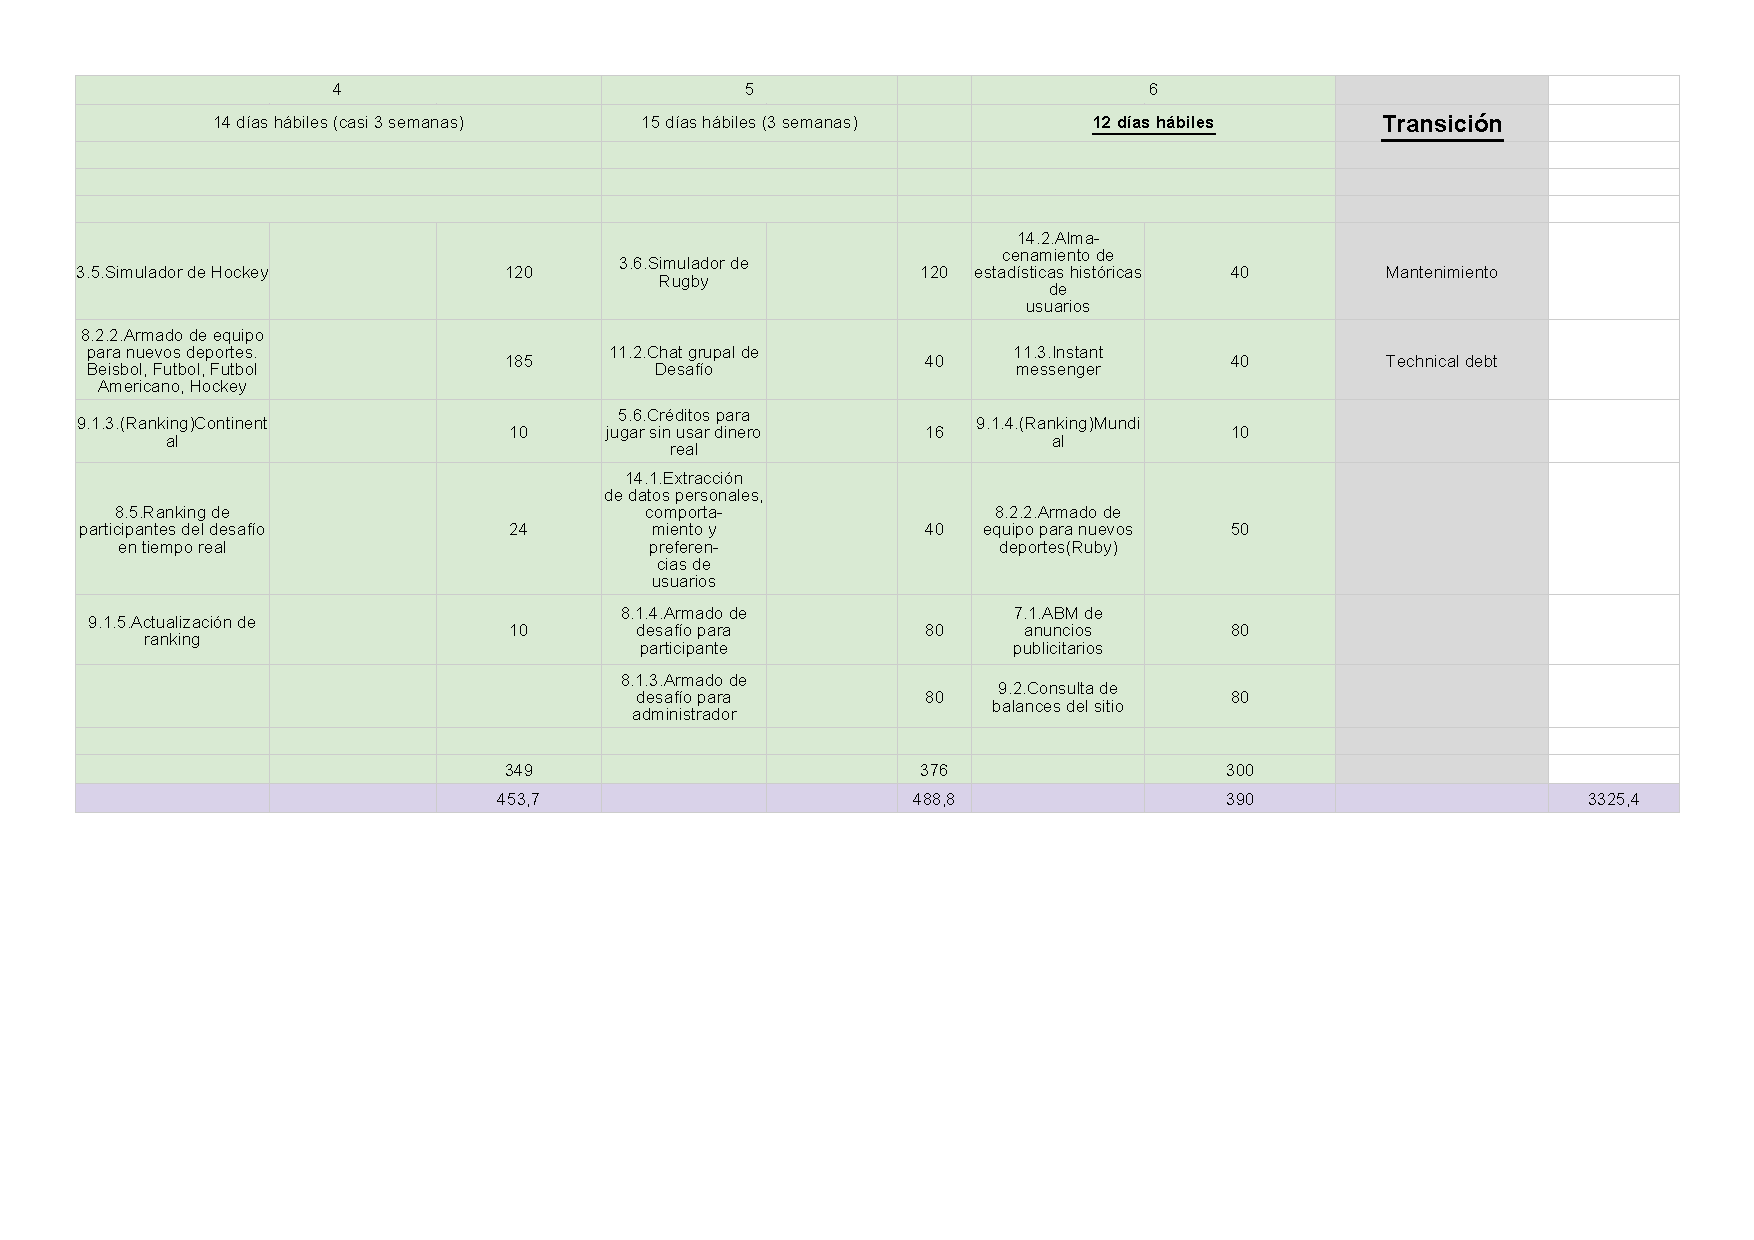
\includegraphics[scale=0.8]{imagenes/construccion-transicion.pdf}
   \caption{División de tareas de las últimas 3 iteraciones de la etapa de 'Construcción' y 'Transicion'}
\end{figure}

\end{landscape}
\newpage




\subsection{Estimación de Módulos}
A continuación se estima en horas hombre los módulos de nivel 1 y 2 del WBS. La estimación se basa en un grupo de trabajo de 4 recursos de 8 horas cada uno, 20 días por mes. Las horas hombre son las horas totales a consumir entre los 4 recursos sumados. Al final se realiza una sumarización de los números para estimar la duración total del proyecto.

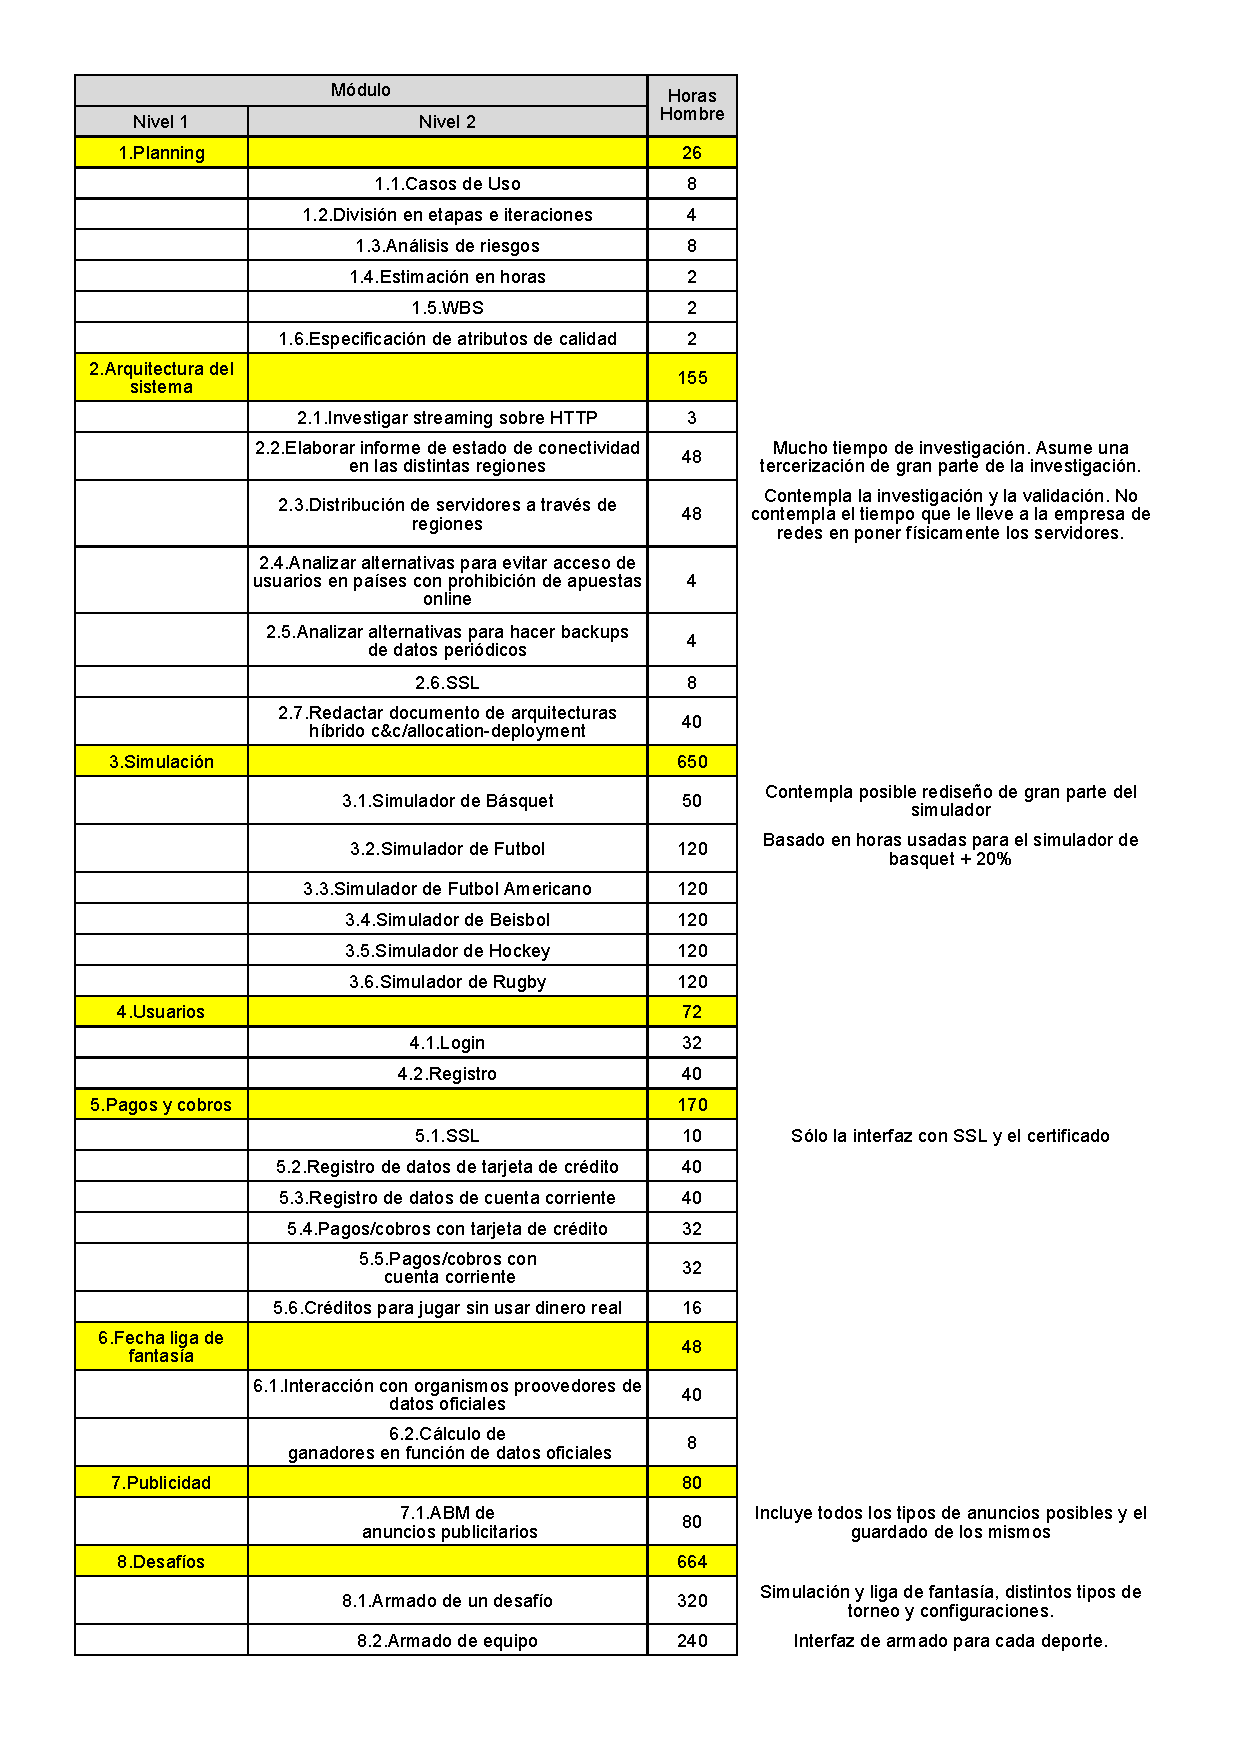
\includegraphics[width=\textwidth, page=1, clip, trim=20 0 20 30]{imagenes/estimacionModulos.pdf}

\newpage
\includegraphics[width=\textwidth, page=2, clip, trim=20 200 20 30]{imagenes/estimacionModulos.pdf}

Como puede observarse, el total estimado es bastante razonable para la magnitud del proyecto. Los tiempos podrían acelerarse si se contratara más gente y se tuviera un grupo de trabajo de 2 o 3 personas en cada módulo. Se estima que en 5 meses el proyecto debería estar funcionando, salvando las demoras que puedan causar los proveedores en responder y realizar su trabajo.
\subsection{Division en etapas e iteraciones}
En el proceso de elaboración se incluyen las tareas relacionadas con la arquitectura del sistema, y se genera una base ejecutable del código sobre la cual se pueda 
empezar a testear dicha arquitectura.

Al mismo tiempo se desarrollan los componentes con un rol central dentro de la arquitectura definida, y los módulos de los casos de uso con más riesgos
de alto impacto a nivel estructural, dejando cada una en una iteración diferente. La idea es construir la arquitectura de forma incremental. La opción a nivel arquitectura propuesta
en cada iteración debe ser compatible con la anterior, y al mismo tiempo solucionar el caso de uso actual.

\begin{figure}[h!]
   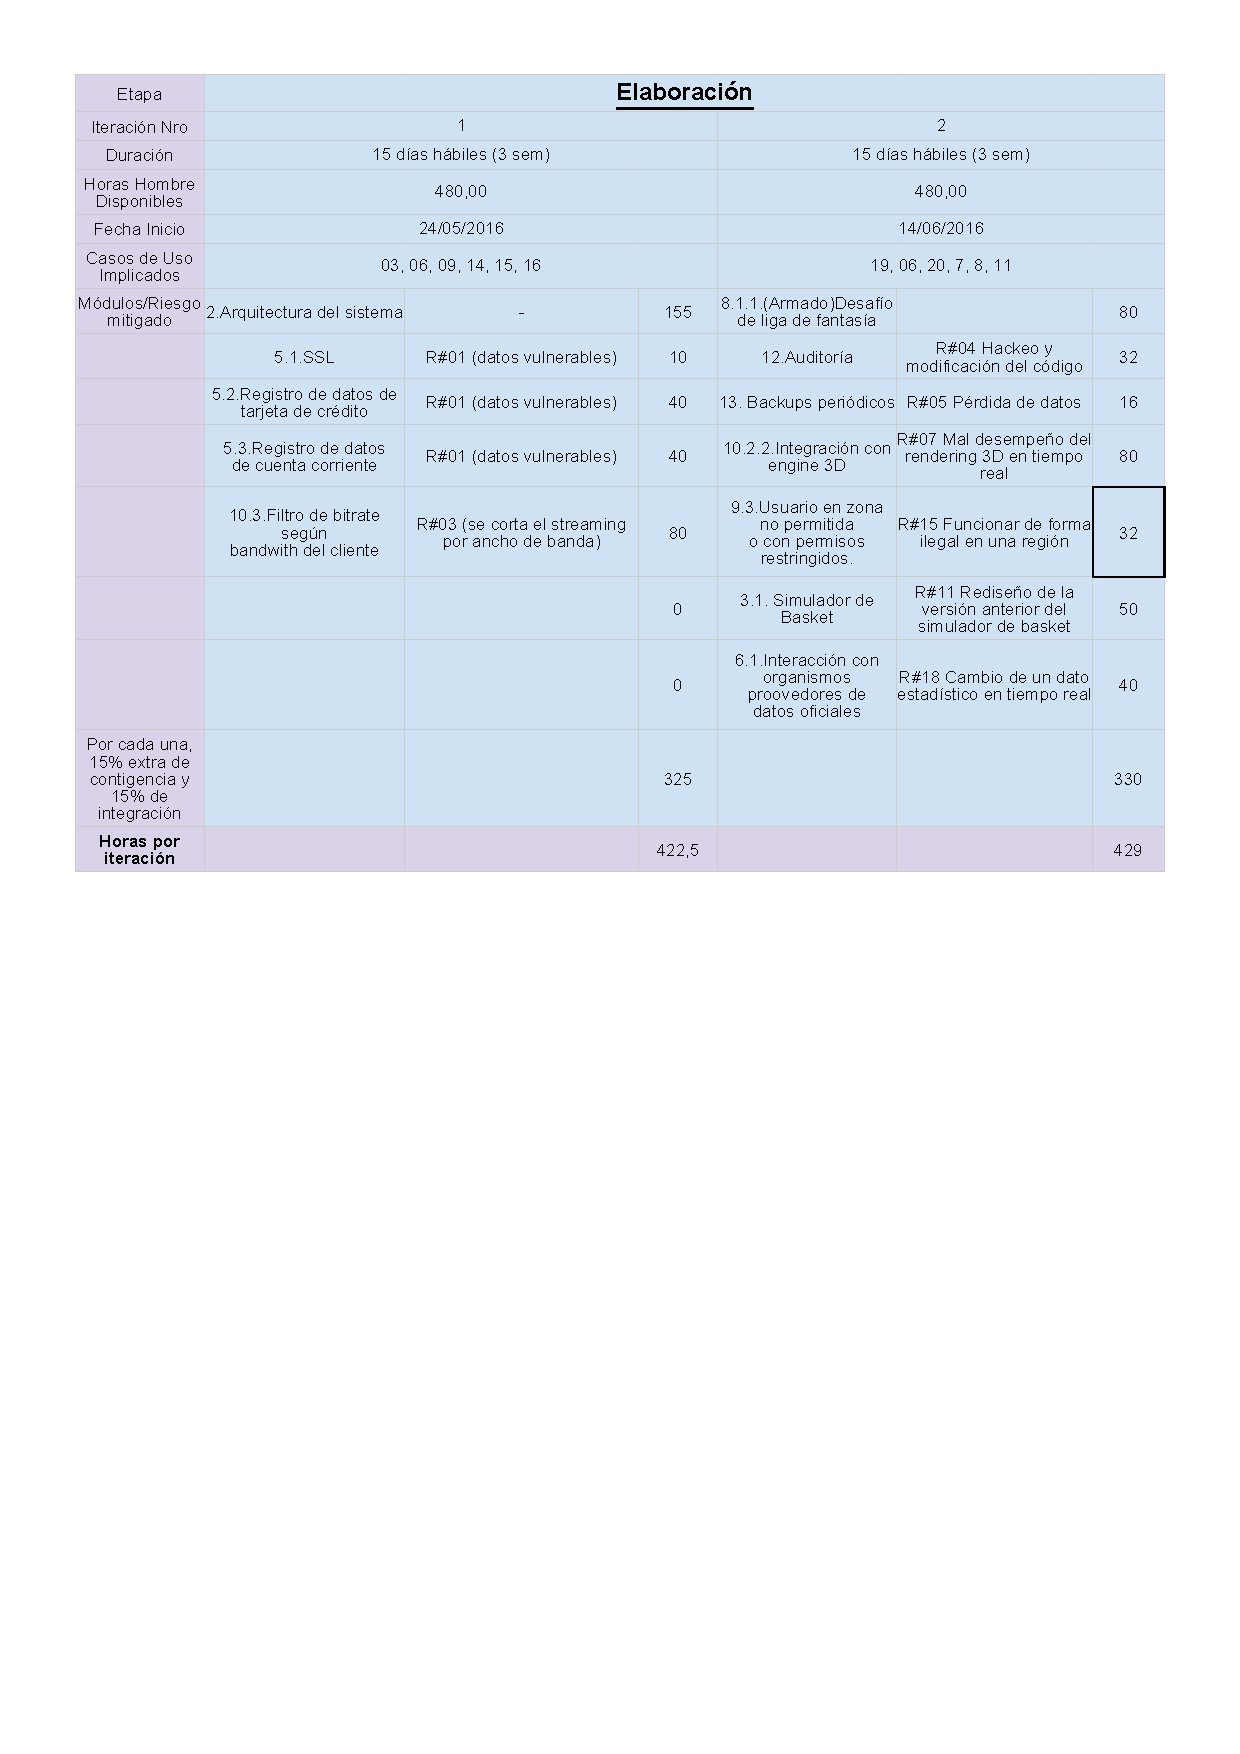
\includegraphics[scale=0.80]{imagenes/etapas-elaboracion.pdf}
   \caption{División de tareas en la etapa de elaboración}
\end{figure}

En la etapa de construcción se desarrollan los módulos y casos de uso faltantes faltantes de forma iterativa incremental. 

Finalmente en la etapa de transición se realizan tareas de mantenimiento.

\newpage
\begin{landscape}

\begin{figure}[h!]
   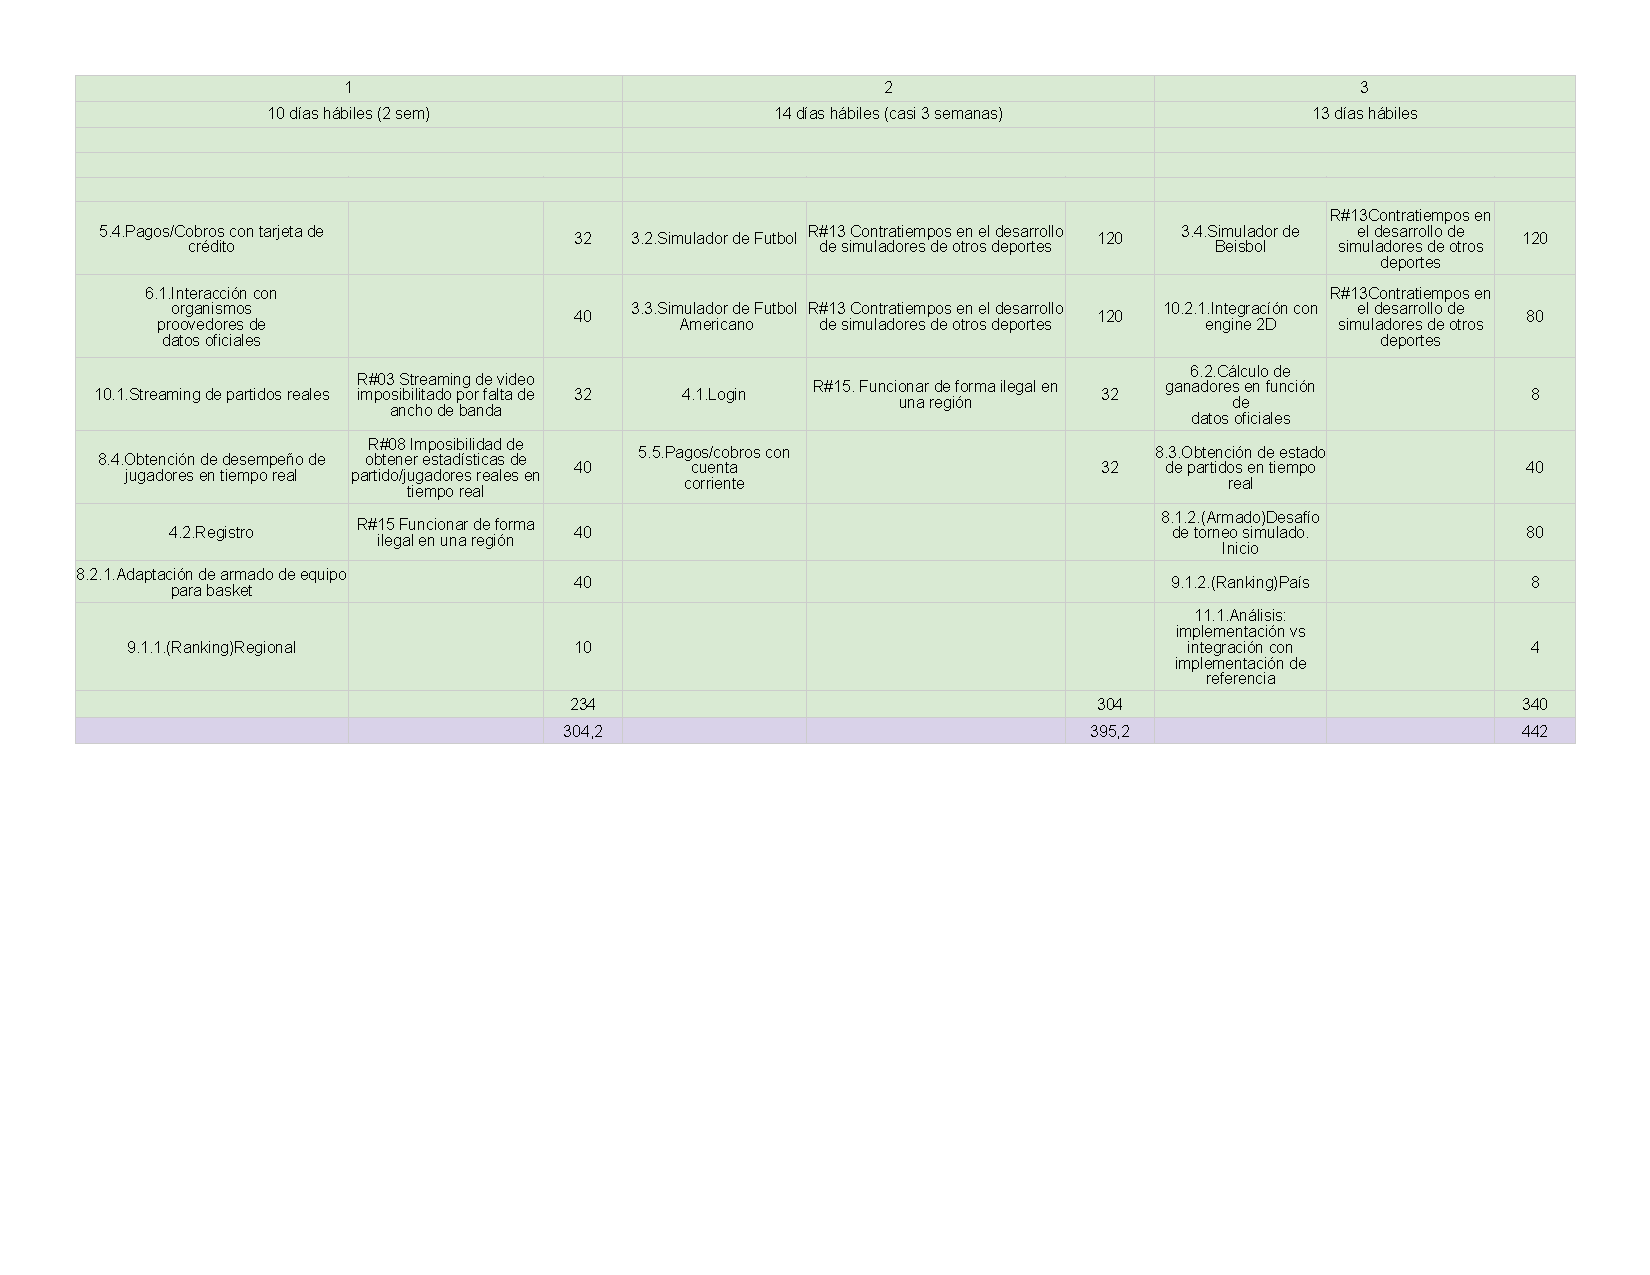
\includegraphics[scale=0.8]{imagenes/construccion123.pdf}
   \caption{División de tareas de las primeras 3 iteraciones de la etapa de 'Construcción'}
\end{figure}

\end{landscape}
\newpage

\newpage
\begin{landscape}

\begin{figure}[h!]
   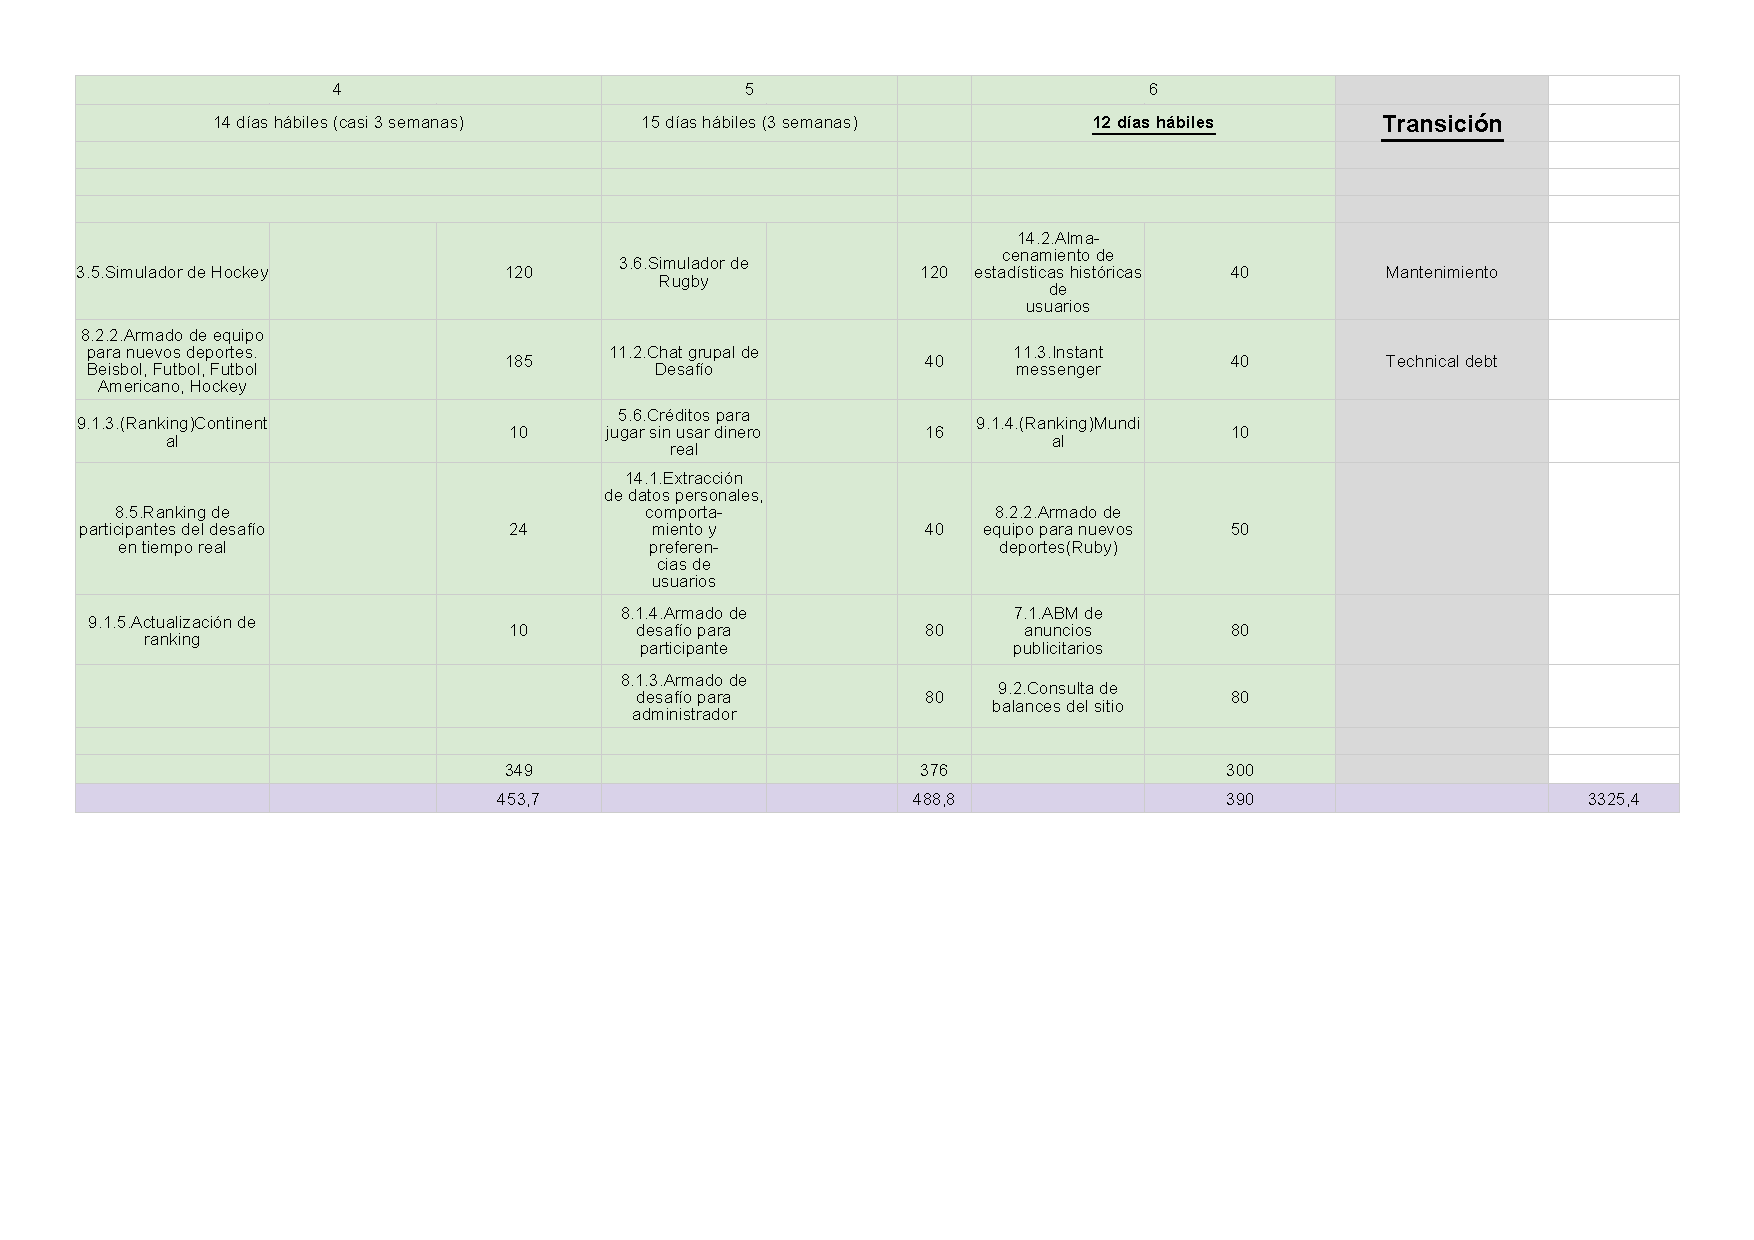
\includegraphics[scale=0.8]{imagenes/construccion-transicion.pdf}
   \caption{División de tareas de las últimas 3 iteraciones de la etapa de 'Construcción' y 'Transicion'}
\end{figure}

\end{landscape}
\newpage




\newpage

\newpage

\bibliographystyle{plain}
\bibliography{tp3}

\end{document}
